\chapter{Cuerdas largas y correspondencia con los agujeros negros}

\lectureoverview{Un agujero negro tiene entropía, por lo que debe poseer grados de libertad microscópicos. Construiremos la explicación más sencilla de esos grados de libertad en teoría de cuerdas: primero contaremos los estados de una cuerda larga excitada y luego variaremos el acoplamiento de cuerda hasta que coincidan las descripciones mediante cuerdas y agujeros negros. Dejaremos deliberadamente la igualdad final como problema para resolver en la próxima clase.}

\section{La entropía exige portadores microscópicos}

Decir que un sistema tiene una entropía grande significa que puede ocultar una gran cantidad de información microscópica. Una bañera de agua caliente puede tener una entropía del orden de \(10^{30}\). Esta afirmación ya nos dice que hay una cantidad enorme de grados de libertad microscópicos, tanto si decidimos examinarlos molécula por molécula como si no. La termodinámica puede determinar la entropía midiendo la energía y la temperatura, pero no identifica los objetos que la portan.

La dinámica de fluidos hace familiar esta distinción. Describe la densidad, la velocidad, la presión y el flujo macroscópico sin referirse a los átomos. Al añadir la termodinámica, se descubre que un fluido tiene entropía. La entropía anuncia una estructura microscópica que las ecuaciones macroscópicas no muestran; plantea una pregunta nueva en vez de responderla.

Los agujeros negros plantean el mismo desafío de forma más aguda. La propuesta de Bekenstein, completada por el cálculo de Hawking, asigna una entropía proporcional al área del horizonte. La relatividad general determina la geometría y su termodinámica, pero no proporciona un inventario de los estados microscópicos. ¿Cuáles son los numerosos objetos pequeños cuyas configuraciones dan cuenta de la ley de áreas? En teoría de cuerdas hay una candidata concreta. El argumento que desarrollaremos aquí es deliberadamente cualitativo: obtiene correctamente la dependencia paramétrica, pero omite las constantes numéricas y el formalismo necesario para un recuento completo de estados.

\section{Tres escalas y una sutileza de notación}

La gravedad introduce una longitud característica, la longitud de Planck,
\begin{equation}
\ell_p=\sqrt{\frac{G_N\hbar}{c^3}}.
\label{eq:l06-planck-si}
\end{equation}

\begin{classroomqa}\audiencequestion{¿Qué combinación de \(G_N\), \(\hbar\) y \(c\) da la longitud de Planck?\lecturetimestamp{00:06:08}}\lecturerresponse{Es \(\sqrt{G_N\hbar/c^3}\), aproximadamente \(10^{-33}\) centímetros. Enseguida fijaremos \(\hbar=c=1\), con lo que la relación se vuelve mucho más sencilla.}\end{classroomqa}

En unidades naturales,
\begin{equation}
\hbar=c=1,
\qquad
G_N=\ell_p^2.
\label{eq:l06-planck-area}
\end{equation}
Así, la constante de Newton tiene dimensiones de área. Por eso un área dividida por \(G_N\) es adimensional y puede representar una entropía.

La teoría de cuerdas tiene una segunda longitud, \(\ell_s\). Si calentamos una cuerda o la ponemos en un estado muy excitado, oscila en muchas escalas. En esta imagen elemental, la escala mínima característica es la longitud de cuerda. Podemos considerar \(\ell_s\) como el tamaño asociado a una unidad elemental de oscilación de la cuerda.

La tercera cantidad es el acoplamiento adimensional de cuerda \(g_s\). Controla la escisión y la unión: una cuerda puede estrangularse hasta dividirse en dos, o una cuerda excitada puede emitir un cuanto de cuerda cerrada.

\begin{classroomqa}\audiencequestion{¿Cuál es el significado físico del acoplamiento de cuerda?\lecturetimestamp{00:09:20}}\lecturerresponse{Controla la probabilidad de una interacción de cuerdas, como la escisión cuando una cuerda se cruza consigo misma. Más precisamente, \(g_s\) es la amplitud de interacción; la probabilidad o la tasa correspondiente comienza en orden \(g_s^2\).}\end{classroomqa}

La excitación emitida de cuerda cerrada sin masa puede ser un gravitón. En este sentido, \(g_s\) desempeña un papel análogo al de la carga eléctrica: es el factor asociado a un vértice de interacción.\editorialnote{En esta clase se alterna entre llamar a \(g_s\) probabilidad y amplitud. En teoría de perturbaciones es el acoplamiento al nivel de las amplitudes; las probabilidades y las tasas contienen su cuadrado.}

\section{Por qué la gravedad depende del cuadrado del acoplamiento \texorpdfstring{\(g_s^2\)}{}}

Consideremos primero la imagen del intercambio en electromagnetismo. Un objeto cargado emite un fotón con un factor \(e\), y un segundo objeto lo absorbe con otro factor \(e\). Por tanto, la amplitud de intercambio contiene \(e^2\). No se trata de una historia literal de proyectiles clásicos, pero sí muestra correctamente cómo interviene el acoplamiento.

\begin{figure}[htbp]\centering
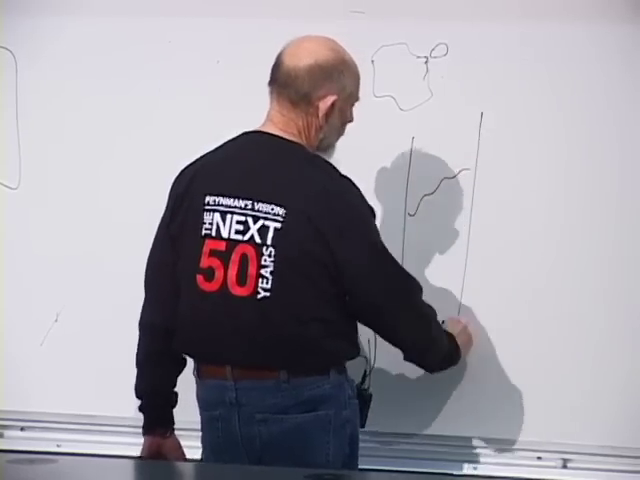
\includegraphics[width=0.72\textwidth]{lecture_06_figure_03.png}\caption{Los diagramas de intercambio completados en la pizarra: hay un acoplamiento en la emisión y otro en la absorción.}\lectureframe{00:11:30.000}\end{figure}

La versión de teoría de cuerdas sustituye el fotón por un gravitón y la carga eléctrica por \(g_s\). Un factor acompaña a la emisión y otro a la absorción, de modo que la intensidad de la interacción gravitatoria escala como \(g_s^2\).

A grandes distancias, la misma interacción debe reproducir la ley de fuerza de Newton,
\begin{equation}
F_{\mathrm{grav}}\sim G_N\frac{M_1M_2}{r^2}.
\end{equation}
Las masas y la dependencia inversa del cuadrado describen las fuentes y la propagación; aquí nos interesa el acoplamiento que las multiplica.

\begin{figure}[htbp]\centering
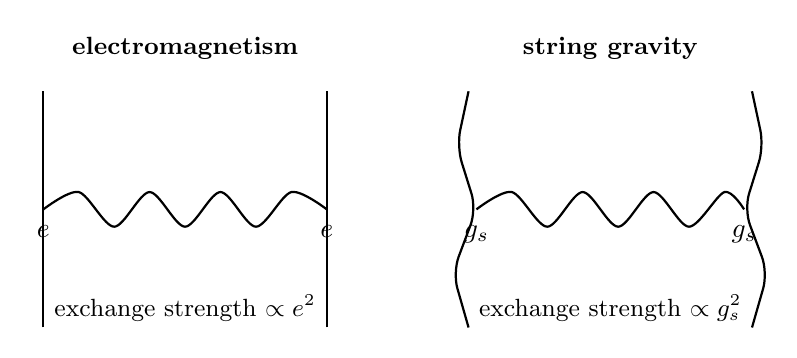
\begin{tikzpicture}[x=1cm,y=1cm]
  \node[font=\small\bfseries] at (1.8,3.55) {electromagnetism};
  \draw[line width=0.8pt] (0,0) -- (0,3);
  \draw[line width=0.8pt] (3.6,0) -- (3.6,3);
  \draw[line width=0.8pt] plot[smooth] coordinates {(0,1.5) (0.45,1.72) (0.9,1.28) (1.35,1.72) (1.8,1.28) (2.25,1.72) (2.7,1.28) (3.15,1.72) (3.6,1.5)};
  \node[below] at (0,1.42) {\(e\)};
  \node[below] at (3.6,1.42) {\(e\)};
  \node[font=\small] at (1.8,0.25) {exchange strength \(\propto e^2\)};
  \node[font=\small\bfseries] at (7.2,3.55) {string gravity};
  \draw[line width=0.8pt,rounded corners=6pt] (5.4,0) -- (5.2,0.7) -- (5.5,1.5) -- (5.25,2.3) -- (5.4,3);
  \draw[line width=0.8pt,rounded corners=6pt] (9,0) -- (9.2,0.7) -- (8.9,1.5) -- (9.15,2.3) -- (9,3);
  \draw[line width=0.8pt] plot[smooth] coordinates {(5.5,1.5) (5.95,1.72) (6.4,1.28) (6.85,1.72) (7.3,1.28) (7.75,1.72) (8.2,1.28) (8.65,1.72) (8.9,1.5)};
  \node[below] at (5.5,1.42) {\(g_s\)};
  \node[below] at (8.9,1.42) {\(g_s\)};
  \node[font=\small] at (7.2,0.25) {exchange strength \(\propto g_s^2\)};
\end{tikzpicture}\caption{La analogía del recuento de acoplamientos. Cada extremo del cuanto intercambiado aporta un factor de interacción.}\end{figure}

Esta observación casi determina la constante de Newton. El acoplamiento \(g_s\) es adimensional, mientras que, en cuatro dimensiones, \(G_N\) tiene dimensiones de longitud al cuadrado. La única longitud microscópica disponible es \(\ell_s\); por tanto,
\begin{equation}
G_N\sim g_s^2\ell_s^2.
\label{eq:l06-newton-string}
\end{equation}
Al combinar esto con la ecuación~\eqref{eq:l06-planck-area}, se obtiene
\begin{equation}
\ell_p\sim g_s\ell_s.
\label{eq:l06-planck-string}
\end{equation}

\begin{figure}[htbp]\centering
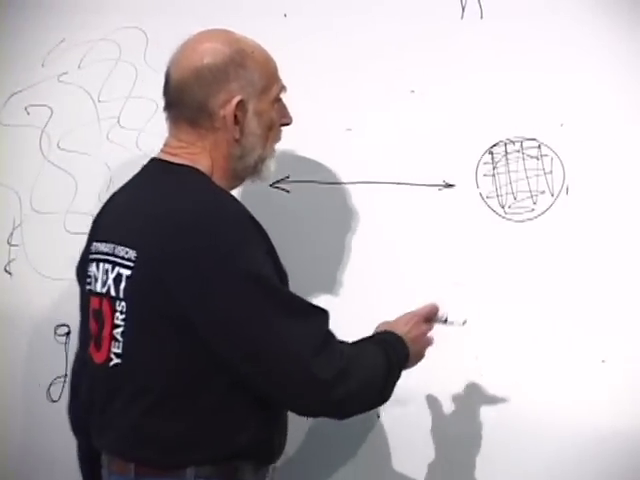
\includegraphics[width=0.72\textwidth]{lecture_06_figure_04.png}\caption{Las relaciones básicas que se conservan en la pizarra: \(\ell_p^2=G_N\) y \(\ell_p\sim g_s\ell_s\).}\lectureframe{00:15:45.000}\end{figure}

La ecuación~\eqref{eq:l06-newton-string} es la relación simplificada que usaremos a lo largo de esta clase.\editorialnote{En una teoría de cuerdas compactificada, la constante de Newton efectiva en cuatro dimensiones también depende del volumen de compactificación y de convenciones de orden unidad. La clase omite esos datos para aislar la dependencia de escala de la correspondencia.}

\begin{classroomqa}\audiencequestion{¿Es \(g_s\) mayor o menor que uno, y cuál de las longitudes es mayor?\lecturetimestamp{00:16:00}}\lecturerresponse{Trabajaremos a acoplamiento débil, \(g_s<1\). Entonces, \(\ell_p\sim g_s\ell_s\) implica que la longitud de cuerda es mayor que la longitud de Planck. El acoplamiento fuerte requiere otra descripción, que aquí no necesitamos.}\end{classroomqa}

\section{El recuento de los agujeros negros}

Si omitimos la constante de Boltzmann y los factores numéricos, la entropía de Bekenstein--Hawking es
\begin{equation}
S_{\mathrm{BH}}=\frac{A}{4G_N}sim\frac{A}{G_N}sim\frac{A}{\ell_p^2}.
\label{eq:l06-bh-area}
\end{equation}
El factor \(1/4\) es exacto en la fórmula semiclásica, pero no desempeñará ningún papel en este argumento de escala.

\begin{classroomqa}\audiencequestion{¿El subíndice ``BH'' significa agujero negro o Bekenstein--Hawking?\lecturetimestamp{00:16:51}}\lecturerresponse{Para nuestros propósitos puede recordarnos ambas cosas. Lo importante es que la entropía es el área del horizonte medida en unidades del área de Planck.}\end{classroomqa}

Para un agujero negro de Schwarzschild en cuatro dimensiones,
\begin{equation}
R_s=2G_NM,
\qquad
A=4\pi R_s^2.
\end{equation}
Omitiendo \(2\) y \(4\pi\), como hace la clase,
\begin{align}
S_{\mathrm{BH}}
&\sim \frac{R_s^2}{G_N}
\sim \frac{(G_NM)^2}{G_N} \\
&\sim M^2G_N
\sim M^2\ell_p^2.
\label{eq:l06-bh-mass}
\end{align}
Esta es la expresión que compararemos con el recuento de cuerdas.

\section{Una cuerda larga como paseo aleatorio}

Empecemos con una cuerda pequeña y aportémosle energía. Una cuerda genérica muy excitada no permanece como un bucle ordenado. Se convierte en un objeto largo y enredado, como un sedal tras enredarse mal en el carrete. El enredo tiene entropía porque hay una enorme cantidad de configuraciones que, macroscópicamente, parecen iguales.

Para contarlas, reemplacemos el espacio por una retícula cuyos enlaces tienen longitud \(\ell_s\). Los sitios son los vértices, los enlaces son las líneas y las celdas elementales son las plaquetas. Una cuerda se representa mediante una sucesión conexa de enlaces. Este modelo es deliberadamente rudimentario, pero su recuento exponencial de estados capta la dependencia de escala que buscamos.

\begin{figure}[htbp]\centering
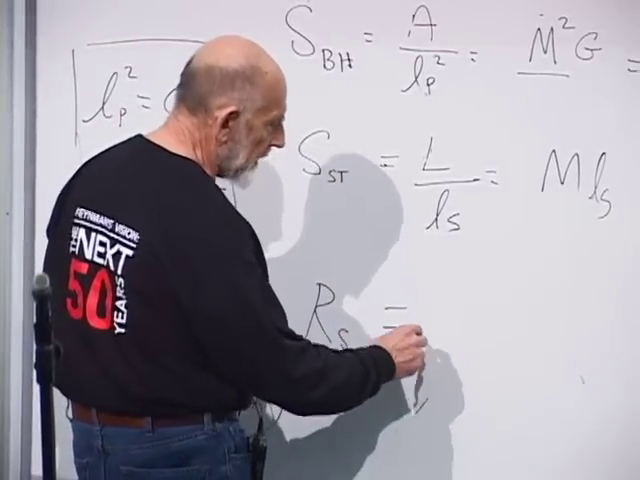
\includegraphics[width=0.72\textwidth]{lecture_06_figure_05.png}\caption{El modelo de retícula bidimensional. El segmento azul marca un paso de la cuerda; en cada sitio se cuentan las cuatro continuaciones posibles.}\lectureframe{00:23:50.000}\end{figure}

\begin{classroomqa}\audiencequestion{¿Cuántas opciones hay en cada paso del paseo simplificado?\lecturetimestamp{00:22:43}}\lecturerresponse{Cuatro en la retícula cuadrada, porque se permite retroceder inmediatamente. En tres dimensiones habría seis. Si se usa otra retícula cambia el número concreto, pero no el hecho de que la cantidad de paseos crece exponencialmente con el número de enlaces.}\end{classroomqa}

Si la cuerda tiene \(n\) enlaces, el recuento del modelo bidimensional es
\begin{equation}
\Omega_n\sim4^n.
\label{eq:l06-walk-count}
\end{equation}
Hay un paseo rectilíneo excepcional, pero es un solo estado entre \(4^n\). Un paseo típico se pliega una y otra vez y ocupa una bola enredada. Para valores grandes de \(n\), casi todas las configuraciones generadas al azar tienen un aspecto cualitativamente similar.

La entropía es el logaritmo del número de configuraciones indistinguibles macroscópicamente:
\begin{equation}
S_{\mathrm{st}}=\log\Omega_n\sim n\log4\sim n.
\label{eq:l06-string-entropy-n}
\end{equation}

\begin{classroomqa}\audiencequestion{¿Por qué la entropía resulta proporcional a \(n\) y no a \(4^n\)?\lecturetimestamp{00:25:39}}\lecturerresponse{La entropía es el logaritmo del número de estados. Así, \(\log(4^n)=n\log4\), y el factor \(\log4\) es una constante de orden unidad que omitiremos.}\end{classroomqa}

Si \(L\) es la longitud de contorno, obtenida siguiendo la cuerda de un extremo al otro, entonces
\begin{equation}
n=\frac{L}{\ell_s},
\qquad
S_{\mathrm{st}}\sim\frac{L}{\ell_s}.
\label{eq:l06-string-entropy-length}
\end{equation}
Aquí, \(L\) no es el diámetro de la bola enredada. Es la distancia mucho mayor medida a lo largo de la cuerda.

A continuación, sustituimos la longitud de contorno por la masa. Con \(c=\hbar=1\), la masa tiene dimensiones de inverso de longitud. Por tanto, un enlace del tamaño de una cuerda tiene una masa del orden de
\begin{equation}
m_{\mathrm{link}}\sim\frac{1}{\ell_s}.
\label{eq:l06-link-mass}
\end{equation}

\begin{classroomqa}\audiencequestion{¿Por qué la masa de un enlace debe escalar como \(1/\ell_s\)?\lecturetimestamp{00:29:20}}\lecturerresponse{En estas unidades, la masa es el inverso de una longitud, y \(\ell_s\) es la única longitud disponible. De forma equivalente, una tensión de cuerda del orden de \(1/\ell_s^2\) multiplicada por una longitud de enlace \(\ell_s\) da el mismo resultado.}\end{classroomqa}

La cuerda completa tiene entonces
\begin{equation}
M\sim n m_{\mathrm{link}}
\sim\frac{n}{\ell_s}
\sim\frac{L}{\ell_s^2},
\qquad
L\sim M\ell_s^2.
\label{eq:l06-string-mass}
\end{equation}
Al sustituir en la ecuación~\eqref{eq:l06-string-entropy-length} se obtiene
\begin{equation}
S_{\mathrm{st}}\sim M\ell_s.
\label{eq:l06-string-entropy-mass}
\end{equation}
El paseo por la retícula ignora las restricciones de la hoja de mundo y los coeficientes numéricos, pero el crecimiento exponencial del espectro de cuerdas muy excitadas da la misma escala dominante.\editorialnote{La construcción mediante un paseo aleatorio sirve como recurso mnemotécnico para la densidad de estados de cuerda a niveles altos; no es una discretización literal de una cuerda fundamental.}

\section{La discrepancia que pone en marcha el argumento}

Ahora tenemos las dos respuestas:
\begin{equation}
S_{\mathrm{BH}}\sim M^2\ell_p^2,
\qquad
S_{\mathrm{st}}\sim M\ell_s.
\label{eq:l06-two-entropies}
\end{equation}
Se parecen, pero no son iguales para una masa fija y un acoplamiento arbitrario. La expresión del agujero negro es cuadrática en \(M\); la de la cuerda es lineal. No podemos declarar sin más que una cuerda caliente es un agujero negro sin explicar cómo se conectan ambos regímenes.

\begin{figure}[htbp]\centering
\includegraphics[width=0.78\textwidth]{lecture_06_figure_06.png}\caption{La comparación despejada en la pizarra: arriba, la entropía del agujero negro; abajo, la entropía de la cuerda larga, y a la izquierda se conservan las relaciones entre Planck--cuerda.}\lectureframe{00:33:20.000}\end{figure}

Aquí se detuvo la clase. El suspenso es útil: la discrepancia no refuta la idea, sino que indica que hay que comparar el mismo estado mientras se modifica la intensidad de la gravedad.

\section{Girar el mando del acoplamiento}

Mantengamos fijo \(\ell_s\) e imaginemos que podemos variar \(g_s\). Para \(g_s=0\), las cuerdas no se dividen ni se unen, y la gravedad desaparece porque \(G_N\sim g_s^2\ell_s^2\). En ese caso, un estado suficientemente energético es una cuerda larga que interactúa débilmente.

Aumentemos \(g_s\) lentamente. Las interacciones de cuerdas se vuelven posibles y, lo que es más importante para el argumento actual, la gravedad se intensifica.

\begin{classroomqa}\audiencequestion{Al aumentar \(g_s\), ¿el primer efecto es simplemente que la cuerda se divide en cuerdas más cortas?\lecturetimestamp{00:36:29}}\lecturerresponse{La escisión y la unión se vuelven posibles, pero mantengamos fijo \(\ell_s\) y sigamos el estado de alta entropía. El efecto central es que aumenta \(G_N\), de modo que la autogravedad de la cuerda larga atrae hacia dentro la bola enredada.}\end{classroomqa}

El objeto se contrae y se vuelve más denso. Su energía potencial gravitatoria es negativa, así que la contracción reduce su energía total y, por tanto, su masa.

\begin{classroomqa}\audiencequestion{¿La energía aumenta o disminuye cuando la autogravedad atrae la cuerda?\lecturetimestamp{00:37:48}}\lecturerresponse{Disminuye. La energía de enlace se vuelve más negativa. La masa a lo largo del recorrido no tiene por qué mantenerse constante, aunque sigamos el mismo estado.}\end{classroomqa}

Con el tiempo, el tamaño del objeto se vuelve comparable a su radio de Schwarzschild. A partir de ese punto, la descripción mediante un agujero negro es la más natural. Una excitación inicial mayor alcanza esta condición con un acoplamiento menor, porque un objeto más masivo necesita menos intensidad gravitatoria para formar un horizonte.

\begin{figure}[htbp]\centering
\resizebox{0.95\linewidth}{!}{%
\begin{tikzpicture}[x=1cm,y=1cm,>=Latex]
  \draw[->,line width=0.9pt] (0,0) -- (11,0) node[right] {increasing \(g_s\)};
  \node[draw,rounded corners,align=center,minimum width=2.6cm,minimum height=1.15cm] at (1.8,1.5) {long excited string\\weak self-gravity};
  \node[draw,rounded corners,align=center,minimum width=2.6cm,minimum height=1.15cm] at (5.5,1.5) {correspondence point\\\(R_s\sim\ell_s\)};
  \node[draw,circle,align=center,minimum size=1.8cm] at (9.3,1.5) {black\\hole};
  \draw[->,line width=0.8pt] (3.15,1.5) -- (4.1,1.5) node[midway,above,font=\small] {contracts};
  \draw[->,line width=0.8pt] (6.9,1.5) -- (8.25,1.5);
  \node[font=\small,align=center] at (5.5,-0.65) {same family of states followed slowly;\\binding energy and mass may change};
\end{tikzpicture}}\caption{La trayectoria de correspondencia a \(\ell_s\) fijo. Invertir la flecha transforma el estado de agujero negro en un estado de cuerda larga.}\end{figure}

\begin{classroomqa}\audiencequestion{¿Debemos imaginar que \(g_s\) varía entre cero y uno?\lecturetimestamp{00:40:18}}\lecturerresponse{Sí. El argumento permanece en el régimen de acoplamiento débil. Si \(g_s\) es muy pequeño, el estado debe tener una masa correspondientemente grande antes de convertirse en un agujero negro. No hace falta entrar en el régimen \(g_s>1\), cuyo control teórico es deficiente.}\end{classroomqa}

En este experimento mental, el cambio lento es reversible.

\begin{classroomqa}\audiencequestion{Si reducimos de nuevo el acoplamiento hasta que la gravedad ya no pueda mantener unido el agujero negro, ¿en qué se convierte?\lecturetimestamp{00:41:37}}\lecturerresponse{En una cuerda larga. Cuando la gravedad se anula, todo lo que aparece en esta construcción debe describirse mediante estados de cuerda. Al girar el mando en un sentido, se transforma una cuerda en un agujero negro; al girarlo en el sentido contrario, un agujero negro se transforma en una cuerda.}\end{classroomqa}

A energía total y volumen fijos, la configuración dominante de alta entropía es, esencialmente, una sola cuerda larga en vez de una cantidad enorme de cuerdas cortas. Esto no se demuestra aquí. Es un resultado de la mecánica estadística de las cuerdas cerca del régimen de Hagedorn y volveremos a estudiarlo.

\section{Lo que observa alguien desde el exterior}

¿Dónde está la cuerda cuando el objeto se describe como un agujero negro? En la descripción exterior no desaparece de golpe. El tiempo de Schwarzschild lleva el cruce aparente a tiempos arbitrariamente tardíos, así que los grados de libertad de cuerda se representan como acumulados sobre el horizonte o cerca de él.

\begin{figure}[htbp]\centering
\includegraphics[width=0.72\textwidth]{lecture_06_figure_07.png}\caption{Comparación en la pizarra entre un horizonte macroscópico, donde la estructura a escala de cuerda es una capa tenue, y un horizonte más pequeño cuyo radio se aproxima a la escala del bucle.}\lectureframe{00:45:30.000}\end{figure}

Para \(R_s\gg\ell_s\), el agujero negro es macroscópico y la estructura a escala de cuerda forma apenas una capa delgada en relación con el radio del horizonte. Cuando el radio disminuye y se acerca a \(\ell_s\), pierde sentido distinguir entre un agujero negro suave y una cuerda extendida. Esta es una descripción exterior, basada en un horizonte estirado; no debe confundirse con la afirmación, independiente de las coordenadas, de que la materia en caída nunca cruza un horizonte regular.\editorialnote{La clase emplea la descripción exterior habitual en la complementariedad de los agujeros negros. La expresión ``sobre el horizonte'' designa grados de libertad resueltos en la descripción exterior, no una derivación independiente de su ubicación covariante.}

La transición ocurre cuando
\begin{equation}
R_s\sim\ell_s.
\label{eq:l06-correspondence-radius}
\end{equation}
Por debajo de la escala de cuerda, la geometría de Schwarzschild no puede resolver la estructura que supuestamente la sustenta. Los bucles fluctúan y se alejan del horizonte que habría de formarse, y resulta más apropiado llamar cuerda al estado.

\section{El punto de correspondencia}

Usamos \(R_s\sim G_NM\) en la ecuación~\eqref{eq:l06-correspondence-radius}:
\begin{equation}
G_NM\sim\ell_s.
\end{equation}
A continuación, sustituimos \(G_N\sim g_s^2\ell_s^2\):
\begin{equation}
M g_s^2\ell_s^2\sim\ell_s,
\qquad
M g_s^2\ell_s\sim1.
\label{eq:l06-correspondence-condition}
\end{equation}

\begin{figure}[htbp]\centering
\includegraphics[width=0.72\textwidth]{lecture_06_figure_08.png}\caption{El álgebra completa de la transición en la pizarra: \(R_s\sim\ell_s\) conduce a la condición adimensional recuadrada \(Mg_s^2\ell_s\sim1\).}\lectureframe{00:49:50.000}\end{figure}

Alguien del público advirtió lo que anticipa esta condición. En el punto de correspondencia,
\begin{align}
S_{\mathrm{BH}}
&\sim M^2\ell_p^2
\sim M^2g_s^2\ell_s^2 \\
&=(M\ell_s)(Mg_s^2\ell_s)
\sim M\ell_s
\sim S_{\mathrm{st}}.
\label{eq:l06-entropy-preview}
\end{align}

\begin{classroomqa}\audiencequestion{¿Las ecuaciones ya implican que las entropías del agujero negro y de la cuerda se vuelven iguales?\lecturetimestamp{00:50:18}}\lecturerresponse{Sí. Justamente hacia eso conduce el cálculo. Ya hemos reunido los elementos en la pizarra, pero la clase aplaza su ensamblaje completo para repasar con cuidado la lógica de la correspondencia.}\end{classroomqa}

La ecuación~\eqref{eq:l06-entropy-preview} es el anticipo algebraico, en una línea, implícito en el intercambio. Establece la dependencia de escala, no el coeficiente exacto \(1/4\). Para obtener igualdades microscópicas exactas hacen falta agujeros negros cuyo análisis esté mejor controlado y construcciones de cuerdas más detalladas.\editorialnote{La clase termina antes de presentar la ecuación~\eqref{eq:l06-entropy-preview} como una derivación completa. La escribimos aquí porque alguien del público señala explícitamente la igualdad y ya han aparecido todas las relaciones necesarias.}

\section{Por qué se conserva la entropía en el proceso}

Queda un ingrediente lógico. Supongamos que variamos suficientemente despacio un parámetro de control, como un campo magnético o \(g_s\), mientras el sistema está aislado y la evolución es reversible. La energía, el tamaño y la energía de enlace pueden cambiar, pero la entropía se conserva:
\begin{equation}
\Delta S=0.
\label{eq:l06-adiabatic-entropy}
\end{equation}
La clase relaciona esto con la conservación de la información. La entropía mide la información que queda oculta en una descripción macroscópica; un cambio lento y reversible del hamiltoniano reorganiza los estados sin eliminar esa información.

\begin{classroomqa}\audiencequestion{¿Para que la entropía sea constante, el recorrido debe evitar una transición de fase?\lecturetimestamp{00:54:01}}\lecturerresponse{Sí, debe ser posible seguir el estado de manera continua. Un sistema finito no presenta una transición de fase termodinámica estrictamente no analítica del tipo que ocurre en el límite de volumen infinito; si el cambio es suficientemente lento, la correspondencia puede tratarse como una transición gradual y suave.}\end{classroomqa}

Aquí se usa «adiabático» en el sentido más estricto de un proceso cuasiestático y reversible. Un proceso adiabático irreversible puede generar entropía; la lentitud y la posibilidad de seguir el estado son esenciales.\editorialnote{La afirmación termodinámica \(\Delta S=0\) exige un proceso adiabático reversible. En mecánica cuántica, la idea correspondiente consiste en seguir el mismo conjunto de estados a medida que cambia un parámetro, sin transiciones entre niveles que no estén controladas.}

\begin{classroomqa}\audiencequestion{¿Por qué una sola cuerda larga debería tener más entropía que varias cuerdas más cortas con la misma masa total?\lecturetimestamp{00:54:44}}\lecturerresponse{Es contraintuitivo, pero el recuento explícito de estados a altas energías favorece una componente de cuerda larga en un volumen fijo. La demostración se aplaza; para el argumento actual solo necesitamos que el agujero negro se transforme en el sector de cuerdas de máxima entropía, y no en un gas diluido de muchísimas cuerdas cortas.}\end{classroomqa}

Por tanto, la estrategia operativa es:
\begin{enumerate}\item Empezar con un agujero negro de masa \(M_0\) y acoplamiento \(g_{s,0}\).
\item Reducir \(g_s\) lentamente mientras se sigue la misma familia de estados de alta entropía.
\item Detenerse en \(R_s\sim\ell_s\), donde la descripción del agujero negro se convierte en una descripción mediante una cuerda larga.
\item Contar los estados de cuerda usando \(S_{\mathrm{st}}\sim M\ell_s\).
\item Transportar esa entropía de vuelta al agujero negro original a lo largo del proceso reversible.
\end{enumerate}

\begin{figure}[htbp]\centering
\includegraphics[width=0.72\textwidth]{lecture_06_figure_09.png}\caption{El principio que se conserva en la pizarra al enunciar la estrategia: un cambio adiabático de \(g_s\) no modifica \(S\).}\lectureframe{00:56:40.000}\end{figure}

La teoría de cuerdas ha producido recuentos de entropía mucho más precisos para agujeros negros cargados, en rotación, supersimétricos, casi extremales y de dimensiones superiores. La discusión del agujero negro neutro de Schwarzschild que presentamos aquí es el argumento aproximado de correspondencia: identifica la densidad paramétrica de estados y la transición física, pero no una degeneración exacta protegida.\editorialnote{La concordancia exacta es más sólida para ciertos agujeros negros especiales cuyos recuentos de estados están protegidos cuando cambia el acoplamiento. Esta clase presenta deliberadamente la versión más sencilla, a orden de magnitud.}

\begin{classroomqa}\audiencequestion{Al anular la gravedad, ¿podría el estado convertirse en dos cuerdas en vez de exactamente en una?\lecturetimestamp{00:58:25}}\lecturerresponse{Hay una probabilidad finita de que se formen unas pocas cuerdas largas, y usar dos en lugar de una no cambia la escala dominante de la entropía. Lo que sí cambiaría el argumento sería la fragmentación en un enorme gas de cuerdas cortas; el recuento estadístico a altas energías no favorece ese resultado.}\end{classroomqa}

El agujero negro es la configuración de máxima entropía que puede concentrarse en una región, y la cuerda larga es el estado correspondiente de alta entropía cuando se elimina la gravedad. Ya hemos conectado ambas descripciones, pero aún no hemos desarrollado un cálculo de precisión. El siguiente paso es repetir el álgebra con cuidado y preguntarnos hasta qué punto es fiable la correspondencia.
